\section{Referencia de la Clase Pago\-View}
\label{classPagoView}\index{PagoView@{PagoView}}
Muestra y administra la ventana con la informaci\'{o}n de un pago.  


{\tt \#include $<$pagoview.h$>$}

Diagrama de herencias de Pago\-View\begin{figure}[H]
\begin{center}
\leavevmode
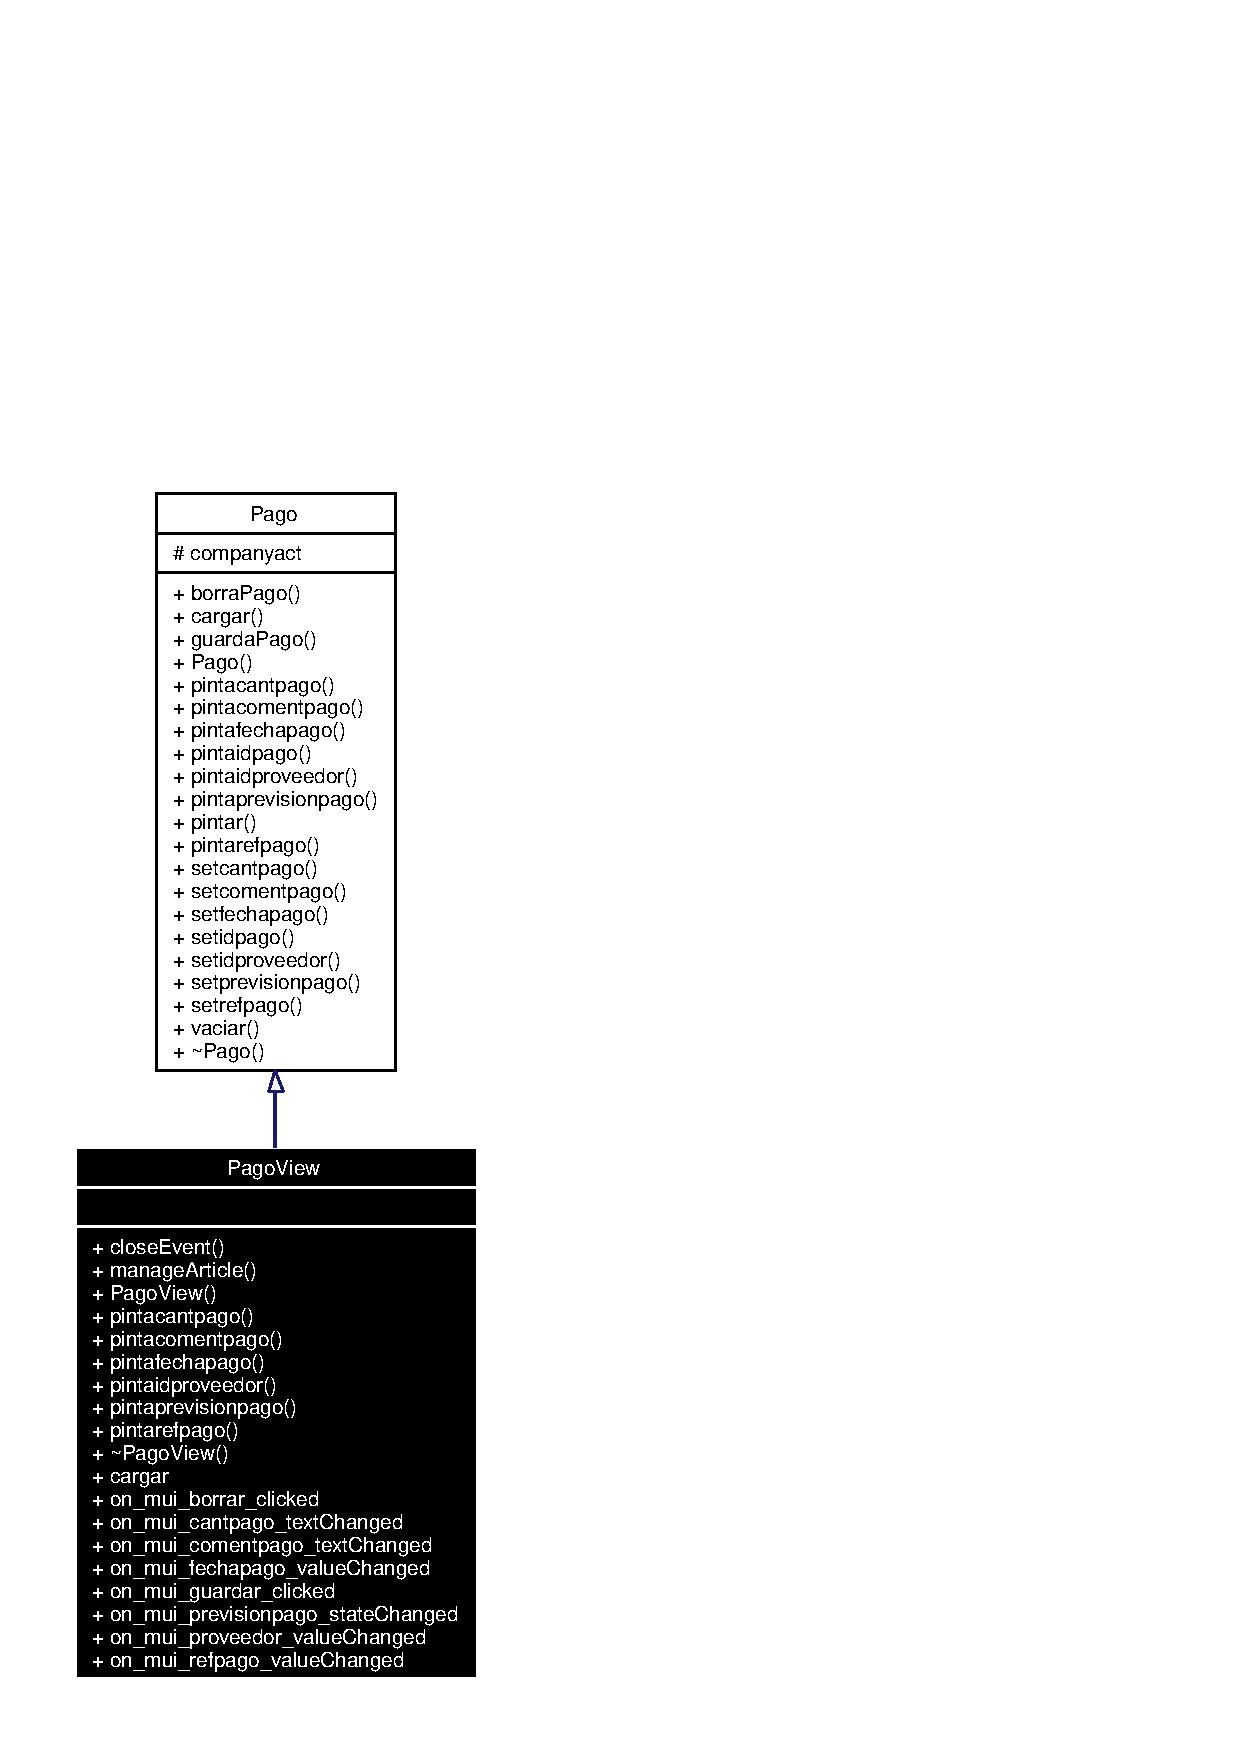
\includegraphics[width=114pt]{classPagoView__inherit__graph}
\end{center}
\end{figure}
Diagrama de colaboraci\'{o}n para Pago\-View:\begin{figure}[H]
\begin{center}
\leavevmode
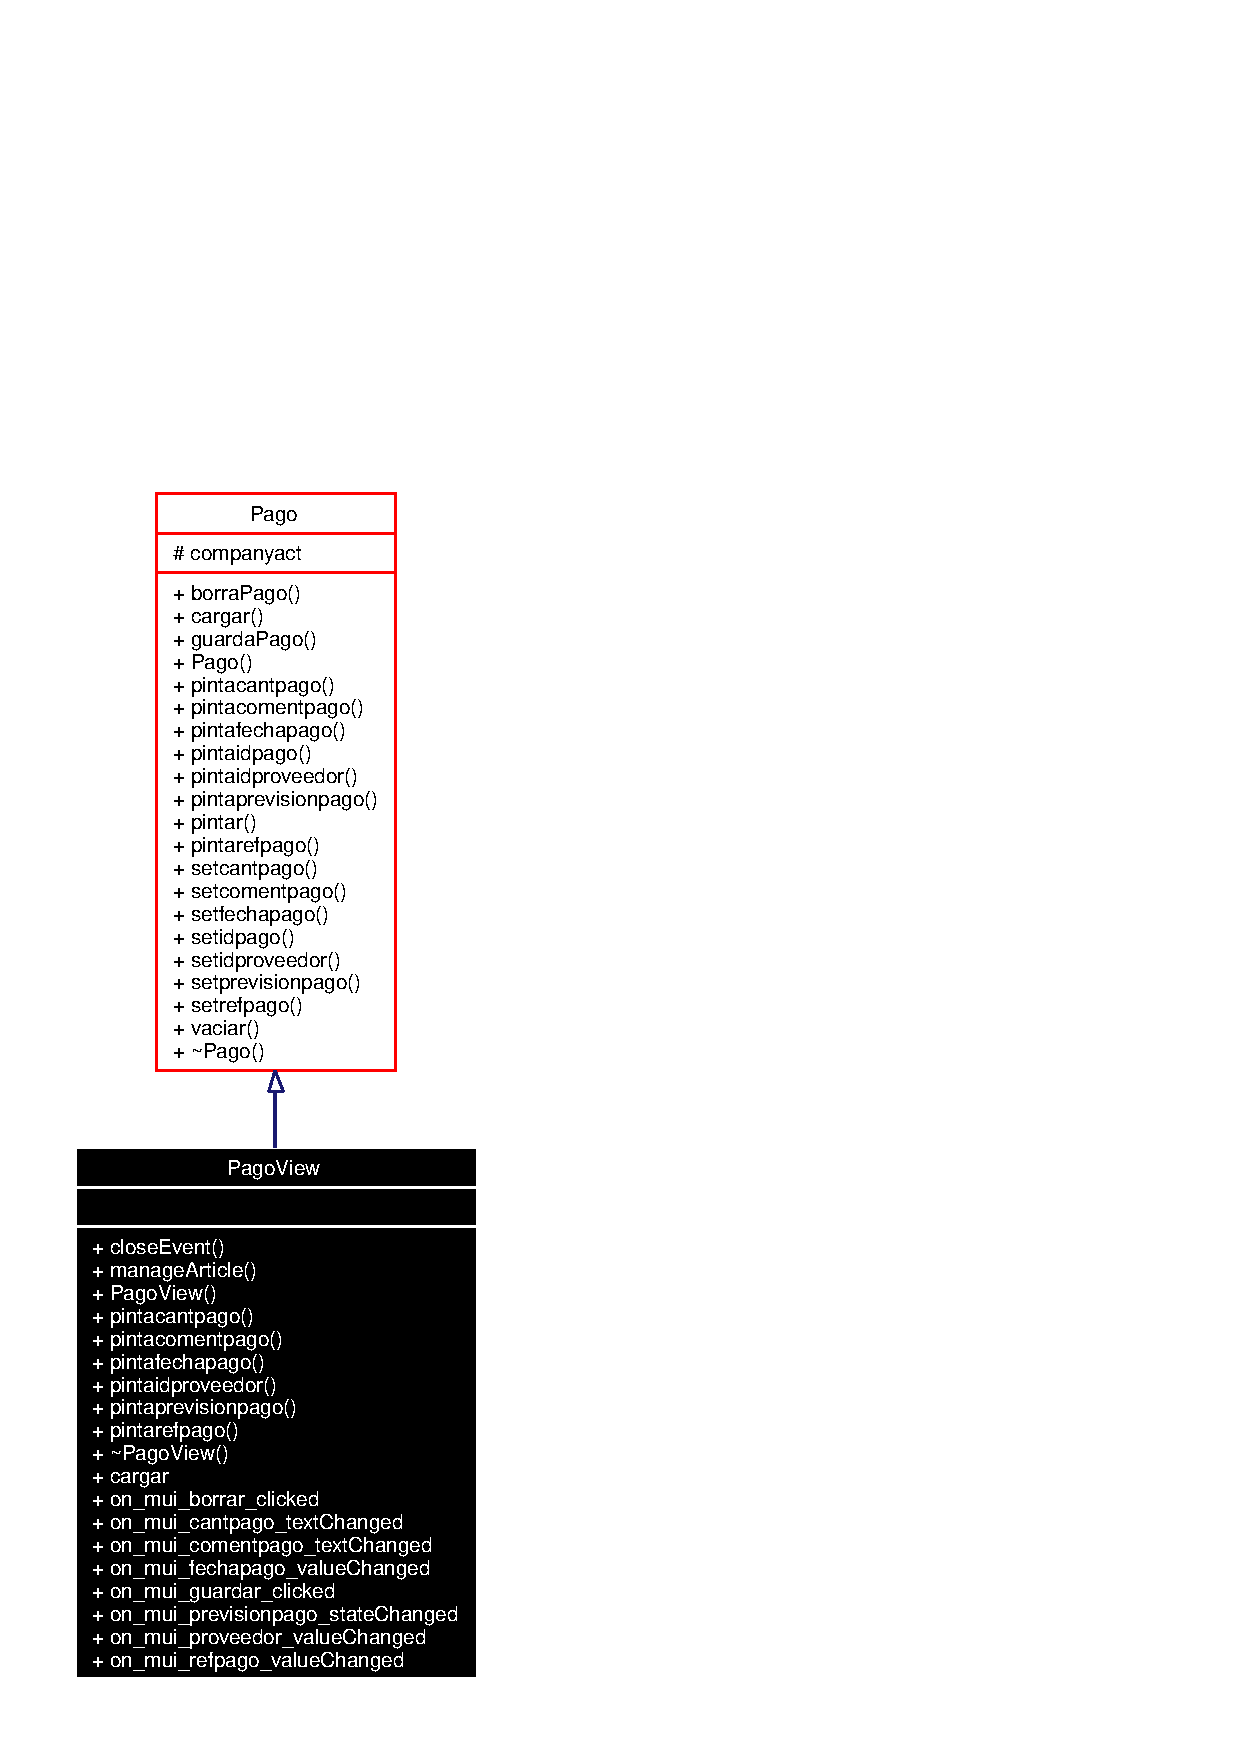
\includegraphics[width=114pt]{classPagoView__coll__graph}
\end{center}
\end{figure}
\subsection*{Slots p\'{u}blicos}
\begin{CompactItemize}
\item 
virtual int {\bf cargar} (QString id)\label{classPagoView_i0}

\begin{CompactList}\small\item\em Esta funcion carga un pago. \item\end{CompactList}\item 
virtual void {\bf on\_\-mui\_\-borrar\_\-clicked} ()\label{classPagoView_i1}

\item 
virtual void {\bf on\_\-mui\_\-cantpago\_\-text\-Changed} (const QString \&str)\label{classPagoView_i2}

\item 
virtual void {\bf on\_\-mui\_\-comentpago\_\-text\-Changed} (const QString \&str)\label{classPagoView_i3}

\item 
virtual void {\bf on\_\-mui\_\-fechapago\_\-value\-Changed} (QString id)\label{classPagoView_i4}

\item 
virtual void {\bf on\_\-mui\_\-guardar\_\-clicked} ()\label{classPagoView_i5}

\item 
virtual void {\bf on\_\-mui\_\-previsionpago\_\-state\-Changed} (int i)\label{classPagoView_i6}

\item 
virtual void {\bf on\_\-mui\_\-proveedor\_\-value\-Changed} (QString id)\label{classPagoView_i7}

\item 
virtual void {\bf on\_\-mui\_\-refpago\_\-value\-Changed} (const QString \&str)\label{classPagoView_i8}

\end{CompactItemize}
\subsection*{M\'{e}todos p\'{u}blicos}
\begin{CompactItemize}
\item 
void {\bf close\-Event} (QClose\-Event $\ast$)\label{classPagoView_a0}

\item 
void {\bf manage\-Article} (int)\label{classPagoView_a1}

\item 
{\bf Pago\-View} ({\bf company} $\ast$, QWidget $\ast$)
\item 
void {\bf pintacantpago} (QString id)\label{classPagoView_a3}

\item 
void {\bf pintacomentpago} (QString id)\label{classPagoView_a4}

\item 
void {\bf pintafechapago} (QString id)\label{classPagoView_a5}

\item 
void {\bf pintaidproveedor} (QString id)\label{classPagoView_a6}

\item 
void {\bf pintaprevisionpago} (QString id)\label{classPagoView_a7}

\item 
void {\bf pintarefpago} (QString id)\label{classPagoView_a8}

\end{CompactItemize}


\subsection{Descripci\'{o}n detallada}
Muestra y administra la ventana con la informaci\'{o}n de un pago. 



\subsection{Documentaci\'{o}n del constructor y destructor}
\index{PagoView@{Pago\-View}!PagoView@{PagoView}}
\index{PagoView@{PagoView}!PagoView@{Pago\-View}}
\subsubsection{\setlength{\rightskip}{0pt plus 5cm}Pago\-View::Pago\-View ({\bf company} $\ast$ {\em comp}, QWidget $\ast$ {\em parent})}\label{classPagoView_a2}


Usurpamos la identidad de mlist y ponemos nuestro propio widget con sus cosillas. 

La documentaci\'{o}n para esta clase fu\'{e} generada a partir de los siguientes archivos:\begin{CompactItemize}
\item 
pagoview.h\item 
pagoview.cpp\end{CompactItemize}
